\chapter{Program Counter Register}

During the course of this semester, we will build a 64-bit computer.  To do this, we will make a synthesizable machine in Verilog, a common hardware description language (HDL).  

A computer runs a program by executing individual instructions in sequential order.  The instructions are stored in memory and are accessed by their memory address.  During each clock cycle, an instruction is fetched from memory and executed on the processor.  The memory address of the next instruction to fetch is stored in a register called the Program Counter (PC).  During Lab 1, we will build and test the Program Counter register.  In Lab 2, we build an incrementer (to count to the next instruction) and a mux (to select between the incremented count or a new starting value).   

\section{Program Counter Register}

In order to make the Program Counter, we are going to make a Verilog module that explains how to build a register (a D flip-flop).  Let me unpack the previous sentence:
\begin{enumerate}
	\item Verilog is a Hardware Description Language (HDL).
	\item We write Verilog code to tell Vivado how we want our register module to behave.
	\item Vivado reads our Verilog code and synthesizes a realizable digital hardware design that meets the behavior that we specified.  Thank you Vivado!
	\item Vivado also simulates the behavior of the hardware, allowing you to test your design without building/programming hardware.
\end{enumerate}   
Consider the Verilog code in Listing~\ref{code:register}.  It is made up of three sections: 
\begin{enumerate}
	\item Header - this code includes a file name definitions.vh which contains information necessary for the program to run.
	\item Port list (also known as interface) - specifies the signals coming into or going out of the module.  In this case, there are three inputs and one output.
	\item Body (also known as implementation) - describes the functionality of the module.
\end{enumerate}

\Verilog{Verilog code to make a register.}{code:register}{../code/1_fetch/register.v}

The first part is the header.  We will use this same header each time.  It tells the Verilog compiler to get all the data from a file called definitions.vh.  The extension vh is a Verilog header.  We use this to specify common pieces of data we will use across our design, so that all the components we build will be consistent.  By putting them in one file, we make it easier to maintain, and prevent mistakes that can happen easily by having multiple copies of these basic pieces of data.  For our first lab, one item that we will be using from definitions.vh is WORD (set to 64), which is the size (in bits) of the memory addresses in our computer.  Note that if we build things based around WORD, rather than the number 64, we can just change the value of WORD in the file and get a computer with a different size with a couple key strokes.

The second part is the port list or interface.  In this area we specify what signals are coming in (input), going out (output), or could go either direction (inout).  Ports can be defined as either "wire" or "reg".  This can be confusing to some students.  Think of it this way: 
\begin{enumerate}
	\item Wire
	\begin{enumerate}
		\item A wire is just a conductor that connects one component or module to another.
		\item The value on a wire can only be changed by using combinational logic (as opposed to sequential logic).
		\item It has no memory, meaning that the value on the wire is driven by the results of combinational logic at that particular moment.
		\item Module inputs are always wires.
		\item Module outputs can be wires or regs.
	\end{enumerate}
	\item Reg
	\begin{enumerate}
		\item A reg more closely resembles a variable in software programming languages.
		\item A value of a reg can only be set by using sequential logic.
		\item A reg has memory, meaning that the value of the reg will remain the same until a sequential logic element updates it.
		\item You can directly set a reg to a value using a procedural assignment.
		\item Regs can be used internally in a module (neither input nor output), or they can be used as module outputs.  They cannot be used as module inputs. 
	\end{enumerate}
\end{enumerate}

\begin{figure}
	\caption{Module Diagram.}\label{fig:modulediagram}
	\begin{center}
		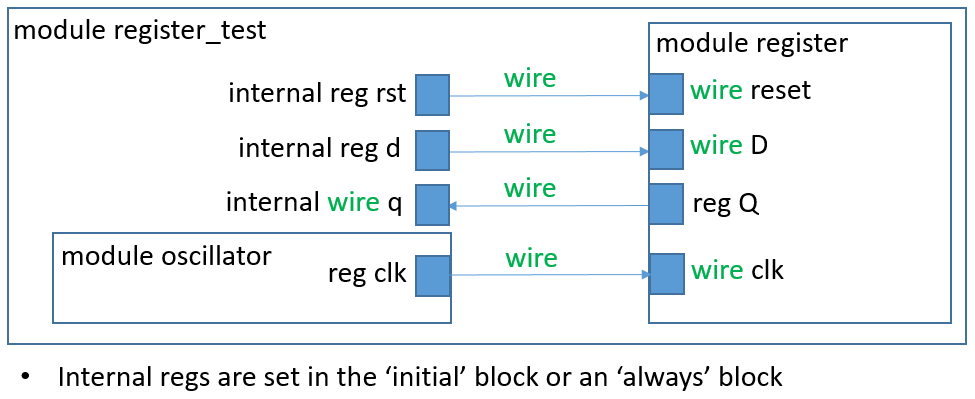
\includegraphics[width=4.75in]{../images/register_test_module_diagram.png}
	\end{center}
\end{figure}

If you don't specify anything for the port type, you will get a wire - it is the default.  In our case we have four signals: three inputs (always wires), and one output that is a register.  The first two inputs are single-bit wires.  One is the clock, which specifies the timing, and the other is reset, which clears the contents of the register (makes them zero).  The final input is the value we want to store in memory, and I have called it D, following the convention of digital logic.  D has multiple bits that are numbered from WORD-1 down to 0.  Thus the leftmost bit is 63 in this case, and the rightmost bit is 0\footnote{If you want to be technical this is called little endian, since the little end (the least significant or unit bit) is going into the first memory location (bit 0).  If you reversed the order by putting the 0 first and the WORD-1 last it would be big endian, since the big end (most significant bit) would go in the lowest addressed bit.}.  The output Q (also the digital logic conventional name) is a register (it will hold its value) and should also be of size WORD and follow the same bit order as the input D.

To help clarify this, please examine Figure~\ref{fig:modulediagram}, which shows the interconnection of the modules in this lab.

The final section is the body or implementation.  It is composed of a single thread of code, that will keep running (hence always).  It will run one time every time there is a positive edge (0 to 1 transition) for either the clock or reset.  Reset has higher priority, so if reset is asserted the register is cleared (Q is set to zero), otherwise the value of D is stored it Q.  That is it.  A nice, simple module.  Please note that the provided register module is fully operational.  You do not need to modify it.

\section{Testbench}

We now want to test our register module using System Verilog.  System Verilog is very similar to Verilog, but it adds the ability to verify that we get the results that we are expecting.  To test the register module, we need to tell the simulator to build a copy (instantiate) of the register module, and then we will need to supply the inputs and evaluate the outputs to verify that the module works correctly.  Consider the testbench in Listing~\ref{code:register_test}.

\Verilog{System Verilog code to test a register.}{code:register_test}{../code/1_fetch/register_test.sv}

When evaluating this testbench module (register\_test), notice that there are no ports.  A testbench is providing all the signals to simulate the inputs to the unit under test (UUT) and thus does not need ports.  This is how Verilog finds a top level simulation module - there are no ports.  The clock signal will be driven by a module named oscillator, which will give us a square wave with period CYCLE, which is another constant defined in our definitions.vh file.  The code thus makes an oscillator and a register, then runs the 'initial' section (it runs once at the start then never again).

This initial section of the testbench follows a relatively simple pattern:
\begin{enumerate}
	\item The inputs to the register module are set to particular values.
	\item The system delays for some amount of time.  For instance, a one cycle delay is inserted with \#CYCLE.
	\item The value of cr (correct result) is set to the output value that you expect to get from the register module.
	\item The value and size of cr are compared with the value and size of ar (actual result).  The actual result is the output of your register module.  I provide (in "verification\_functions.sv", included at the top of the testbench) the verify function and a few other functions that allow us to easily verify the behavior of our system.  Each time verify is called, it keeps track of whether the test passed (ar == cr) or failed (ar != cr).
	\item At the end of the testbench, the final\_result function is called to report the results of the test.  This function will show the number of passing and failing test cases.
\end{enumerate}  


\begin{figure}
\caption{Timing diagram.}\label{fig:registertiming}
\begin{center}
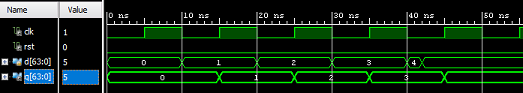
\includegraphics[width=4.75in]{../images/register_test_timing_diagram.png}
\end{center}
\end{figure}

\section{Your Assignment}

You are to:
\begin{enumerate}
\item Evaluate the testbench in Listing~\ref{code:register_test}.  It is not an exhaustive testbench, but it tests a number of cases that commonly occur in our system.  Note that you should not change the input values or timing of the testbench, nor should you add additional test cases to the testbench.
\item Create an Expected Results Table for your testbench.  An example Expected Results Table is at ARM-Lab/testfiles/Lab1\_Register\_ExpectedResultsTable.xlsx.  The idea behind the Expected Results Table is that you identify how you think the system should operate.  If you don't know how it should work, you will not know whether your simulation results are correct.  The Expected Results Table should have a row for each signal in your simulation results (and the row order should match between your Expected Results Table and Simulation Results).  The table should also have a column for each test point in the testbench.  These test points are the points in time that correspond to the 'verify' function calls in the testbench.  To complete the table, fill in each cell with the expected value.  Note that you don't need to show the clk signal in the Expected Results Table.  See the Lab1 Expected Results Table Excel file in the testfiles section of my git repository.
\item The provided testbench does not set the cr to the correct value, therefore causing your test to fail.  Your job now is to take the values from your expected results table and enter these values in the testbench as the cr (correct result).
\item Run a behavioral simulation.  Evaluate the timing diagram and verify that it matches the Expected Results Table.  Also evaluate the printouts in the Tcl Console window in Vivado.  These printouts will indicate the number of passes and fails that occurred in the test.  If you chose the correct cr values and all tests pass, then your module is verified to work properly.   
\item Rather than writing a lab report, please produce a landscape mode single page PDF called Lab1\_lastname.pdf that includes (in this order):
	\begin{enumerate}
		\item Your name and the lab number.
		\item A snip (using the Snipping Tool) of your Expected Results Table.
		\item A snip of the Simulation Results.  Make sure to show all values in decimal form and don't cut off the signal names on the left.  
		\item A snip of the test results from the Tcl Console.  This snip should show the entire log from BEGIN TEST RESULTS to END TEST RESULTS.
		\item I have included a sample in the testfiles directory of my git repository. 
	\end{enumerate}
\item Upload Lab1\_lastname.pdf file to Canvas.
\item Zip up your ARM-Lab directory and submit it on Canvas as well.  I will run your code against my correct testbench to verify that your code and testbench work correctly.  Since I give you working register.v code in this lab, this is pretty easy.  In future labs, you must create your own module code.
\end{enumerate} 
